\clearpage
\phantomsection

\setcounter{chapter}{0}
\chapter[{Tổng quan về Học tăng cường và Game Roguelike}]{Tổng quan về Học tăng cường và Game Roguelike}

Chương này trình bày các khái niệm nền tảng được sử dụng trực tiếp trong đề tài: Học tăng cường, mô hình tác nhân--môi trường, thuật toán PPO, hàm lợi thế GAE, đặc trưng của game hành động Roguelike và các kỹ thuật hỗ trợ huấn luyện như intrinsic motivation, LSTM và curriculum learning. Trọng tâm của chương không phải là khảo sát toàn bộ lịch sử RL, mà là xây dựng nền tảng cần thiết để giải thích thiết kế CombatAgent, môi trường bản đồ sinh theo thủ tục và các thí nghiệm ablation ở các chương sau.

\section{Học tăng cường}
\subsection{Khái niệm cơ bản}

Học tăng cường (Reinforcement Learning -- RL) là một nhánh của học máy trong đó tác nhân học cách ra quyết định thông qua tương tác với môi trường. Tại mỗi bước thời gian, tác nhân quan sát trạng thái hiện tại, chọn một hành động, nhận phần thưởng và chuyển sang trạng thái mới. Mục tiêu cuối cùng là tìm một chính sách hành động giúp tối đa hóa tổng phần thưởng tích lũy trong dài hạn.

Một bài toán RL thường được mô hình hóa dưới dạng Quy trình Quyết định Markov (Markov Decision Process -- MDP), ký hiệu bởi bộ $(S,A,P,R,\gamma)$:

\begin{itemize}
    \item $S$: không gian trạng thái hoặc không gian quan sát mà tác nhân nhận được từ môi trường.
    \item $A$: không gian hành động mà tác nhân có thể chọn.
    \item $P(s_{t+1}|s_t,a_t)$: xác suất chuyển trạng thái của môi trường.
    \item $R(s_t,a_t)$: hàm phần thưởng phản ánh mức độ tốt của hành động.
    \item $\gamma$: hệ số chiết khấu, quyết định mức độ ưu tiên phần thưởng tương lai.
\end{itemize}

Trong đề tài này, $S$ tương ứng với vector quan sát 207 chiều của CombatAgent; $A$ là không gian hành động rời rạc nhiều nhánh $(3,3,3,9)$; $R$ là hàm thưởng kết hợp giữa tín hiệu kết quả như gây sát thương, tiêu diệt kẻ địch, dọn phòng và các tín hiệu định hình như tiếp cận mục tiêu hoặc căn hướng tấn công. Mục tiêu huấn luyện là tối đa hóa kỳ vọng tổng thưởng:

\begin{equation}
    J(\pi_\theta) = \mathbb{E}_{\tau \sim \pi_\theta}
    \left[\sum_{t=0}^{T}\gamma^t r_t\right],
\end{equation}

trong đó $\pi_\theta(a|s)$ là chính sách được tham số hóa bởi mạng nơ-ron, còn $\tau$ là quỹ đạo tương tác của tác nhân trong một episode.

\subsection{Vòng lặp tác nhân--môi trường}

\begin{figure}[H]
    \centering
    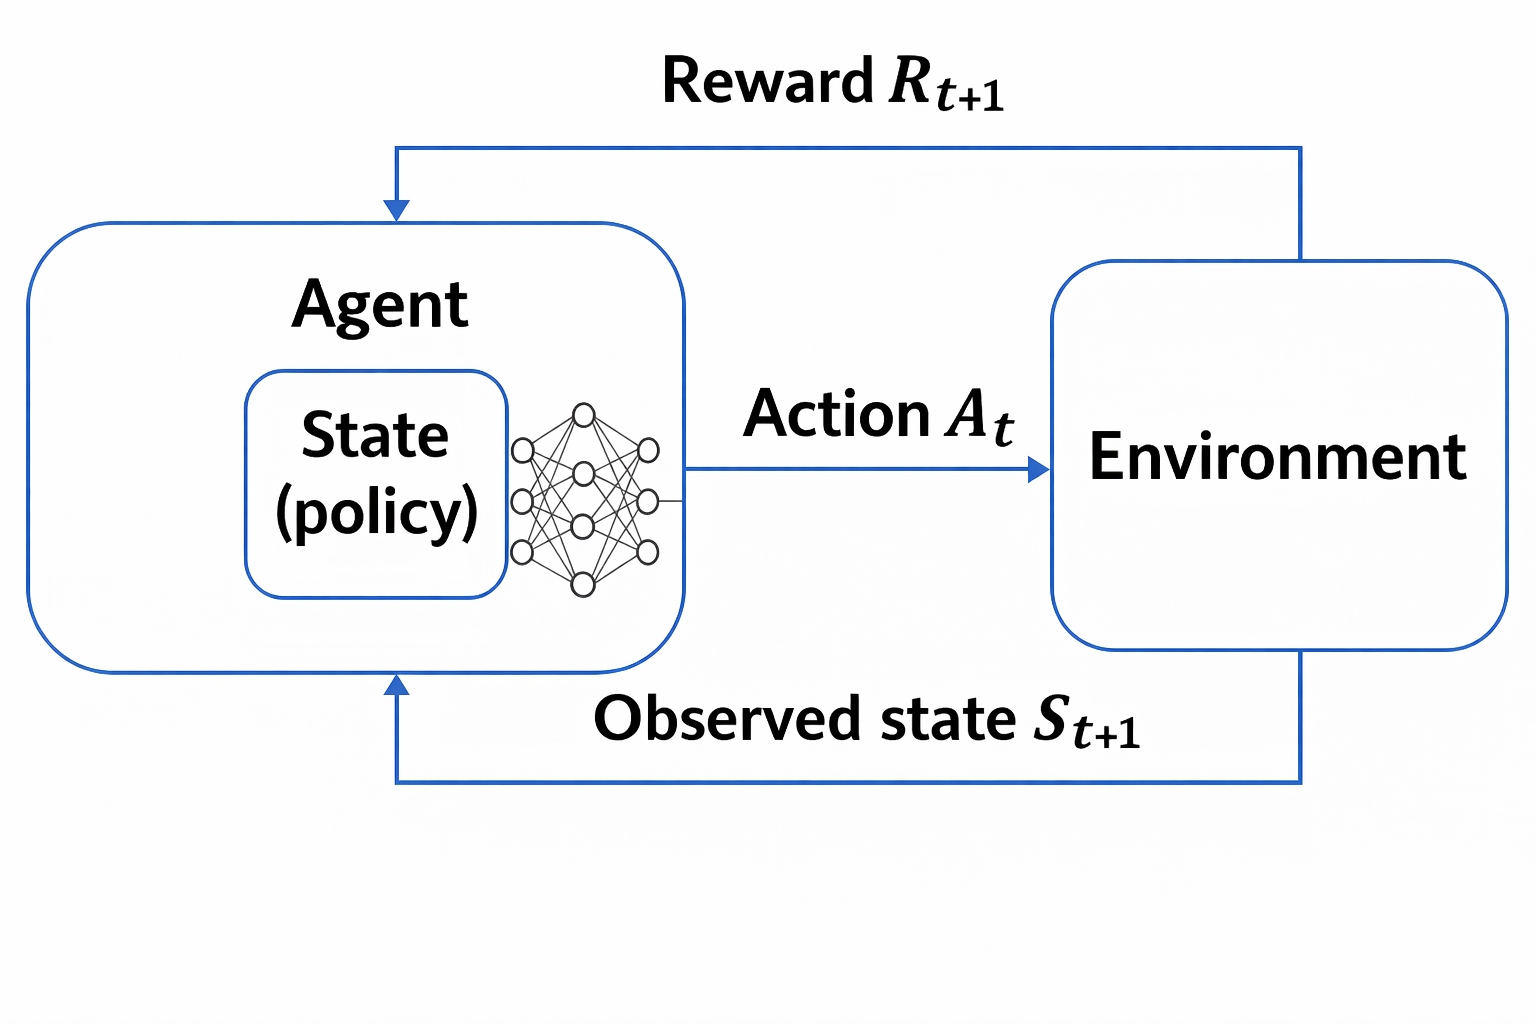
\includegraphics[width=0.9\linewidth]{figures/RL_Loop.png}
    \caption{Chu trình tương tác giữa tác nhân và môi trường trong học tăng cường}
    \label{fig:rl_loop}
\end{figure}

Hình~\ref{fig:rl_loop} mô tả vòng lặp cơ bản của RL. Môi trường cung cấp quan sát $s_t$, tác nhân chọn hành động $a_t$, sau đó môi trường cập nhật trạng thái và trả về phần thưởng $r_t$. Khác với học có giám sát, dữ liệu huấn luyện không có sẵn từ đầu mà được sinh ra trong quá trình tác nhân tương tác với môi trường.

Đặc điểm này phù hợp với game, vì game cung cấp một hệ thống phản hồi rõ ràng: hành động tốt có thể làm tăng điểm, gây sát thương hoặc hoàn thành màn; hành động kém có thể khiến nhân vật nhận sát thương, mắc kẹt hoặc thất bại. Tuy nhiên, nó cũng tạo ra ba khó khăn chính:

\begin{itemize}
    \item \textbf{Khám phá và khai thác:} tác nhân cần thử hành động mới để tìm chiến thuật tốt hơn, nhưng cũng phải khai thác những hành vi đã học được.
    \item \textbf{Phần thưởng trễ:} một hành động hiện tại có thể chỉ thể hiện giá trị sau nhiều bước, ví dụ như né đạn để sống sót đủ lâu rồi mới tiêu diệt được kẻ địch.
    \item \textbf{Dữ liệu phụ thuộc theo thời gian:} các mẫu dữ liệu liên tiếp trong RL có tương quan mạnh vì hành động trước ảnh hưởng trực tiếp tới trạng thái sau.
\end{itemize}

Các khó khăn này xuất hiện rõ trong môi trường của đề tài: tác nhân phải vừa tiếp cận mục tiêu, vừa tránh đạn và tường, vừa chọn thời điểm tấn công hoặc dash trong một phòng có bản đồ và vị trí sinh thay đổi theo episode.

\section{Học tăng cường sâu cho điều khiển game}
\subsection{Từ Q-Learning đến Deep RL}

Q-Learning là một thuật toán nền tảng của RL, trong đó tác nhân học giá trị $Q(s,a)$ cho từng cặp trạng thái--hành động. Với các môi trường nhỏ, giá trị này có thể lưu bằng bảng tra cứu. Tuy nhiên, cách tiếp cận dạng bảng nhanh chóng trở nên không khả thi khi số trạng thái lớn hoặc liên tục.

Trong game hành động Roguelike của đề tài, trạng thái bao gồm máu, vị trí tương đối của kẻ địch, đạn, tường, hồi chiêu, hướng di chuyển và nhiều thông tin khác. Ngay cả khi đã rút gọn thành vector 207 chiều, số cấu hình trạng thái có thể xuất hiện vẫn rất lớn. Do đó, phương pháp bảng không phù hợp; cần dùng mạng nơ-ron để xấp xỉ chính sách hoặc hàm giá trị.

Deep Q-Network (DQN) mở rộng Q-Learning bằng mạng nơ-ron và dùng các kỹ thuật như experience replay, target network để ổn định huấn luyện. DQN phù hợp với nhiều bài toán có không gian hành động rời rạc đơn nhánh. Tuy nhiên, môi trường trong đề tài yêu cầu tác nhân đồng thời chọn nhiều nhóm hành động: di chuyển theo trục X, di chuyển theo trục Y, ý định chiến đấu và hướng ngắm. Vì vậy, một phương pháp tối ưu trực tiếp chính sách như PPO phù hợp hơn với không gian hành động rời rạc nhiều nhánh trong Unity ML-Agents.

\subsection{Actor-Critic}

Các phương pháp Actor-Critic kết hợp hai thành phần:

\begin{itemize}
    \item \textbf{Actor:} sinh ra phân phối xác suất trên các hành động, tức chính sách $\pi_\theta(a|s)$.
    \item \textbf{Critic:} ước lượng giá trị của trạng thái hoặc hành động, thường ký hiệu là $V_\phi(s)$.
\end{itemize}

Actor chịu trách nhiệm quyết định tác nhân nên làm gì, trong khi Critic đánh giá hành động đó tốt hơn hay kém hơn kỳ vọng. Thiết kế này giúp giảm phương sai so với policy gradient thuần túy và phù hợp với các bài toán điều khiển phức tạp. Trong Unity ML-Agents, PPO được triển khai theo hướng Actor-Critic, do đó phù hợp với hệ thống CombatAgent.

\section{Proximal Policy Optimization}
\subsection{Lý do lựa chọn PPO}

Proximal Policy Optimization (PPO) là thuật toán được chọn làm nền tảng huấn luyện trong đề tài \cite{Schulman2017}. Lý do chính là PPO có độ ổn định cao, dễ cấu hình trong Unity ML-Agents và hỗ trợ tốt không gian hành động rời rạc nhiều nhánh. Trong môi trường game hành động Roguelike, chính sách không được thay đổi quá đột ngột sau mỗi lần cập nhật, vì điều đó có thể làm tác nhân mất các hành vi đã học như tiếp cận mục tiêu, né đạn hoặc căn hướng tấn công.

PPO giải quyết vấn đề này bằng cách giới hạn mức thay đổi của chính sách thông qua tỷ lệ xác suất:

\begin{equation}
    r_t(\theta) =
    \frac{\pi_\theta(a_t|s_t)}
    {\pi_{\theta_{\mathrm{old}}}(a_t|s_t)}.
\end{equation}

Nếu $r_t(\theta)$ quá xa 1, chính sách mới đã thay đổi quá nhiều so với chính sách cũ. PPO dùng hàm mục tiêu có cắt ngưỡng để hạn chế cập nhật quá lớn:

\begin{equation} \label{eq:ppo_clip}
    L^{CLIP}(\theta) =
    \hat{\mathbb{E}}_t
    \left[
    \min
    \left(
    r_t(\theta)\hat{A}_t,
    \mathrm{clip}(r_t(\theta),1-\epsilon,1+\epsilon)\hat{A}_t
    \right)
    \right].
\end{equation}

Trong đó $\hat{A}_t$ là lợi thế ước lượng tại bước $t$, còn $\epsilon$ là biên độ cắt. Cơ chế này giữ cho quá trình học nằm trong vùng thay đổi vừa đủ: chính sách vẫn cải thiện, nhưng giảm nguy cơ sụp đổ do cập nhật quá mạnh.

\subsection{Hàm mục tiêu tổng hợp}

Trong thực tế huấn luyện, PPO không chỉ tối ưu chính sách mà còn tối ưu hàm giá trị và khuyến khích khám phá thông qua entropy. Một dạng mục tiêu tổng hợp thường được viết như sau:

\begin{equation} \label{eq:ppo_total}
    L_t(\theta) =
    L_t^{CLIP}(\theta)
    - c_1 L_t^{VF}(\theta)
    + c_2 S[\pi_\theta](s_t).
\end{equation}

Trong đó $L_t^{VF}$ là lỗi của hàm giá trị, còn $S[\pi_\theta]$ là entropy của chính sách. Thành phần entropy đặc biệt quan trọng trong đề tài vì action space $(3,3,3,9)$ có nhiều tổ hợp hành động. Nếu entropy giảm quá sớm, tác nhân có thể hội tụ vào hành vi đơn điệu như chỉ di chuyển, chỉ né hoặc tấn công không đúng thời điểm.

\section{Hàm lợi thế và GAE}

Trong Actor-Critic, hàm lợi thế cho biết một hành động tốt hơn hay tệ hơn mức kỳ vọng tại trạng thái hiện tại:

\begin{equation}
    A(s_t,a_t) = Q(s_t,a_t) - V(s_t).
\end{equation}

Nếu lợi thế dương, hành động đó nên được tăng xác suất trong chính sách; nếu lợi thế âm, xác suất nên giảm. Để ước lượng lợi thế ổn định hơn, PPO thường dùng Generalized Advantage Estimation (GAE). GAE tính lợi thế dựa trên chuỗi sai số TD:

\begin{equation}
    \delta_t = r_t + \gamma V(s_{t+1}) - V(s_t),
\end{equation}

\begin{equation} \label{eq:gae_formula}
    \hat{A}_t^{GAE(\gamma,\lambda)}
    =
    \delta_t
    +(\gamma\lambda)\delta_{t+1}
    + \dots
    +(\gamma\lambda)^{T-t+1}\delta_{T-1}.
\end{equation}

Tham số $\lambda$ điều chỉnh sự cân bằng giữa độ lệch và phương sai. Trong môi trường của đề tài, GAE hữu ích vì phần thưởng có cả thành phần dày như tiếp cận mục tiêu và thành phần thưa như dọn sạch phòng. Cách ước lượng này giúp tín hiệu học ổn định hơn khi tác nhân phải ra quyết định trong các episode có độ dài và cấu trúc khác nhau.

\section{Game Action Roguelike trong phạm vi đề tài}
\subsection{Đặc trưng của môi trường}

Roguelike truyền thống thường gắn với bản đồ sinh ngẫu nhiên, độ khó cao và yêu cầu thích nghi qua nhiều lượt chơi. Đề tài này tập trung vào biến thể hành động góc nhìn từ trên xuống: thời gian trong game diễn ra liên tục, kẻ địch và đạn di chuyển trong không gian 2D, còn tác nhân phải điều khiển nhân vật để sống sót và tiêu diệt kẻ địch.

Tuy nhiên, hệ thống không sử dụng action liên tục trực tiếp. Để phù hợp với Unity ML-Agents và giúp huấn luyện ổn định hơn, điều khiển của CombatAgent được rời rạc hóa thành bốn nhánh hành động $(3,3,3,9)$. Thiết kế này vẫn biểu diễn được các hành vi cần thiết như đứng yên, di chuyển theo tám hướng, tấn công, dash và ngắm theo hướng rời rạc, nhưng giảm độ khó so với việc học trực tiếp vector điều khiển liên tục.

Các đặc trưng quan trọng của môi trường gồm:

\begin{itemize}
    \item \textbf{Bản đồ thay đổi theo episode:} hệ thống sử dụng các text map được sinh bằng PCGNN, sau đó chia thành Easy, Medium và Hard để phục vụ curriculum.
    \item \textbf{Vị trí sinh có thể cố định hoặc ngẫu nhiên:} một số lesson dùng fixed spawn để giảm phương sai ban đầu, sau đó chuyển sang random spawn để tăng độ khó.
    \item \textbf{Chiến đấu thời gian thực:} tác nhân phải xử lý đồng thời kẻ địch, đạn, tường, hồi chiêu và hướng tấn công.
    \item \textbf{Quan sát có cấu trúc:} thay vì ảnh pixel, tác nhân nhận vector 207 chiều mô tả người chơi, kẻ địch, đạn và tường.
    \item \textbf{Phần thưởng kết hợp:} môi trường dùng cả sparse reward cho kết quả chính và shaping reward để dẫn dắt hành vi trung gian \cite{Ibrahim2024}.
\end{itemize}

\subsection{Các thách thức đối với học tăng cường}

Môi trường Action Roguelike trong đề tài tạo ra bốn thách thức chính đối với RL.

\textbf{Thứ nhất, phân phối trạng thái thay đổi mạnh.} Khi bản đồ và vị trí spawn thay đổi, tác nhân không thể chỉ ghi nhớ một đường đi cố định. Chính sách cần học các quy tắc tổng quát hơn, ví dụ như tiếp cận kẻ địch khi an toàn, tránh đạn đang đến gần và không di chuyển vào tường.

\textbf{Thứ hai, hành động có tính phối hợp.} Một quyết định tốt thường không nằm ở một nút bấm đơn lẻ mà ở sự kết hợp giữa hướng di chuyển, hướng ngắm và ý định chiến đấu. Đây là lý do đề tài dùng action space rời rạc nhiều nhánh thay vì một nhánh hành động đơn.

\textbf{Thứ ba, phần thưởng chính khá thưa.} Tín hiệu lớn như tiêu diệt kẻ địch hoặc dọn phòng không xuất hiện liên tục. Nếu chỉ dựa vào các phần thưởng này, tác nhân có thể mất rất nhiều thời gian để khám phá hành vi có ích. Vì vậy, hệ thống bổ sung các shaping reward như tiếp cận mục tiêu, căn hướng tấn công, tấn công hợp lệ và dash hữu ích.

\textbf{Thứ tư, quá trình học dễ bị kẹt ở giai đoạn đầu.} Khi đưa tác nhân trực tiếp vào toàn bộ phân phối Hard, PPO có thể mất nhiều episode chỉ để học các hành vi cơ bản. Do đó, curriculum learning được dùng như một cơ chế tăng độ khó dần, giúp tác nhân học kỹ năng nền trước khi đối mặt với phân phối khó hơn.

\section{Các kỹ thuật hỗ trợ được đánh giá}
\subsection{Intrinsic motivation: ICM và RND}

Intrinsic motivation bổ sung phần thưởng nội tại nhằm khuyến khích tác nhân khám phá các trạng thái mới hoặc khó dự đoán. Trong đề tài, hai hướng được đánh giá là Intrinsic Curiosity Module (ICM) \cite{Pathak2017} và Random Network Distillation (RND) \cite{Burda2018}. Cả hai đều tạo thêm một tín hiệu thưởng phụ $r_t^{int}$ bên cạnh phần thưởng từ môi trường $r_t^{ext}$:

\begin{equation}
    r_t = r_t^{ext} + \alpha r_t^{int},
\end{equation}

trong đó $\alpha$ là hệ số điều chỉnh độ mạnh của phần thưởng nội tại. Điểm khác nhau nằm ở cách định nghĩa $r_t^{int}$.

\textbf{Intrinsic Curiosity Module (ICM).}
ICM đo mức độ mới lạ thông qua sai số dự đoán chuyển trạng thái. Trước hết, trạng thái được đưa qua một bộ mã hóa đặc trưng $\phi(s)$. Sau đó ICM huấn luyện hai mô hình phụ:

\begin{itemize}
    \item \textbf{Inverse model:} dự đoán hành động $a_t$ từ hai đặc trưng liên tiếp $\phi(s_t)$ và $\phi(s_{t+1})$.
    \item \textbf{Forward model:} dự đoán đặc trưng kế tiếp $\hat{\phi}(s_{t+1})$ từ $\phi(s_t)$ và hành động $a_t$.
\end{itemize}

Với không gian hành động rời rạc, inverse loss thường là cross-entropy:

\begin{equation}
    L_{inv} =
    CE\left(a_t,\hat{a}_t\right),
    \quad
    \hat{a}_t =
    g\left(\phi(s_t),\phi(s_{t+1})\right).
\end{equation}

Forward loss được tính bằng sai số bình phương trong không gian đặc trưng:

\begin{equation}
    L_{fwd} =
    \frac{1}{2}
    \left\|
    \hat{\phi}(s_{t+1}) - \phi(s_{t+1})
    \right\|_2^2,
    \quad
    \hat{\phi}(s_{t+1}) =
    f\left(\phi(s_t),a_t\right).
\end{equation}

Phần thưởng nội tại của ICM thường lấy từ forward loss:

\begin{equation}
    r_t^{ICM} =
    \frac{1}{2}
    \left\|
    \hat{\phi}(s_{t+1}) - \phi(s_{t+1})
    \right\|_2^2.
\end{equation}

Quy trình ICM có thể tóm tắt như sau:

\begin{enumerate}
    \item Nhận chuyển tiếp $(s_t,a_t,s_{t+1})$ từ môi trường.
    \item Mã hóa $s_t$ và $s_{t+1}$ thành $\phi(s_t)$ và $\phi(s_{t+1})$.
    \item Dùng inverse model để dự đoán hành động đã gây ra chuyển tiếp.
    \item Dùng forward model để dự đoán đặc trưng của trạng thái kế tiếp.
    \item Lấy sai số dự đoán forward làm phần thưởng khám phá.
\end{enumerate}

Trong bài toán của đề tài, ICM có ý nghĩa vì nó khuyến khích CombatAgent tạo ra các chuyển tiếp trạng thái mới, ví dụ tiếp cận vị trí chiến đấu khác, tương tác với kẻ địch hoặc né các cấu hình đạn khác nhau. Tuy nhiên, do action space của CombatAgent là rời rạc nhiều nhánh $(3,3,3,9)$, inverse model cũng khó hơn: nó phải học quan hệ giữa chuyển trạng thái và tổ hợp hành động di chuyển--chiến đấu--ngắm.

\textbf{Random Network Distillation (RND).}
RND không dự đoán hành động hay chuyển trạng thái. Thay vào đó, RND dùng hai mạng nơ-ron nhận cùng một trạng thái đầu vào: mạng mục tiêu $f$ được khởi tạo ngẫu nhiên và giữ cố định, còn mạng dự đoán $\hat{f}_{\theta}$ được huấn luyện để bắt chước đầu ra của mạng mục tiêu.

Sai số dự đoán được tính như sau:

\begin{equation}
    L_{RND} =
    \left\|
    \hat{f}_{\theta}(s_t) - f(s_t)
    \right\|_2^2.
\end{equation}

Phần thưởng nội tại của RND được lấy trực tiếp từ sai số này:

\begin{equation}
    r_t^{RND} =
    \left\|
    \hat{f}_{\theta}(s_t) - f(s_t)
    \right\|_2^2.
\end{equation}

Quy trình RND có thể tóm tắt như sau:

\begin{enumerate}
    \item Nhận trạng thái hoặc quan sát $s_t$ từ môi trường.
    \item Tính đầu ra của mạng mục tiêu cố định $f(s_t)$.
    \item Tính đầu ra của mạng dự đoán $\hat{f}_{\theta}(s_t)$.
    \item Lấy sai số giữa hai đầu ra làm phần thưởng khám phá.
    \item Huấn luyện mạng dự đoán để giảm sai số trên các trạng thái đã gặp.
\end{enumerate}

Với RND, trạng thái càng ít được gặp thì mạng dự đoán càng chưa học tốt, nên sai số càng cao và agent nhận nhiều phần thưởng nội tại hơn. Khi trạng thái được thăm nhiều lần, sai số giảm dần, làm phần thưởng khám phá tự suy giảm. Vì không cần inverse model, RND thường đơn giản hơn ICM trong các môi trường có action space phức tạp.

\begin{table}[H]
    \centering
    \small
    \caption{So sánh ICM và RND}
    \label{tab:icm_rnd_compare}
    \begin{tabular}{|p{3.1cm}|p{5.0cm}|p{5.0cm}|}
        \hline
        \textbf{Tiêu chí} & \textbf{ICM} & \textbf{RND} \\
        \hline
        Nguồn tín hiệu & Sai số dự đoán chuyển trạng thái trong không gian đặc trưng. & Sai số bắt chước mạng mục tiêu ngẫu nhiên cố định. \\
        \hline
        Phụ thuộc hành động & Có, vì forward model dùng $a_t$ và inverse model dự đoán $a_t$. & Không trực tiếp; chủ yếu đo độ mới lạ của trạng thái. \\
        \hline
        Thành phần học thêm & Encoder, inverse model và forward model. & Mạng mục tiêu cố định và mạng dự đoán. \\
        \hline
        Điểm mạnh & Khuyến khích các chuyển tiếp trạng thái mà agent chưa hiểu rõ. & Đơn giản, ổn định hơn khi action space nhiều nhánh. \\
        \hline
        Rủi ro trong đề tài & Inverse model có thể khó học với action space $(3,3,3,9)$. & Có thể thưởng cho trạng thái mới nhưng không nhất thiết hữu ích cho chiến đấu. \\
        \hline
    \end{tabular}
\end{table}

Hai kỹ thuật này được đưa vào các run ablation để kiểm tra xem phần thưởng nội tại có giúp PPO vượt qua giai đoạn khám phá ban đầu hay không. Việc so sánh ICM và RND cũng giúp phân biệt hai kiểu khám phá: khám phá dựa trên chuyển tiếp có điều kiện hành động và khám phá dựa trên độ mới lạ của trạng thái.

\subsection{Bộ nhớ LSTM}

Long Short-Term Memory (LSTM) là kiến trúc mạng hồi tiếp có khả năng giữ thông tin qua nhiều bước thời gian \cite{Hochreiter1997}. Trong môi trường game hành động, bộ nhớ có thể hữu ích khi quyết định hiện tại phụ thuộc vào lịch sử gần đây, ví dụ hướng di chuyển của đạn, thời điểm hồi chiêu hoặc trạng thái kẻ địch vừa rời khỏi vùng quan sát.

Đề tài triển khai các cấu hình PPO kết hợp LSTM để kiểm tra giả thuyết rằng thông tin lịch sử giúp cải thiện chính sách. Các kết quả định lượng ở Chương~4 cho thấy LSTM là một hướng đáng phân tích, nhưng không tạo ra cải thiện đột phá trong các run đã thực hiện.

\subsection{PCGNN và sinh bản đồ bằng neuroevolution}

Procedural Content Generation (PCG) là hướng tạo nội dung game bằng thuật toán thay vì thiết kế hoàn toàn thủ công. Trong phạm vi đề tài, nội dung cần sinh là bản đồ dạng lưới gồm tường, sàn, vị trí sinh người chơi và vị trí sinh kẻ địch. Cách biểu diễn này phù hợp với game Roguelike vì mỗi episode có thể dùng một cấu hình phòng khác nhau nhưng vẫn giữ được luật chơi và cấu trúc quan sát ổn định.

PCGNN (Procedural Content Generation using NEAT and novelty search) là một phương pháp sinh màn chơi bằng cách tiến hóa mạng nơ-ron thay vì tối ưu trực tiếp từng bản đồ riêng lẻ \cite{Beukman2022}. Ý tưởng chính là dùng NEAT để tiến hóa một mạng sinh cấp độ: tại mỗi ô của bản đồ, mạng nhận thông tin ngữ cảnh cục bộ xung quanh ô đó cùng một số đầu vào ngẫu nhiên, sau đó dự đoán loại tile cần đặt. Sau giai đoạn tiến hóa offline, mạng tốt nhất có thể sinh nhiều bản đồ mới rất nhanh và có thể áp dụng cho các kích thước khác nhau mà không cần huấn luyện lại từ đầu.

Đối với đề tài này, PCGNN không được dùng trực tiếp trong vòng lặp huấn luyện Unity theo thời gian thực. Thay vào đó, PCGNN được dùng như một bước tiền xử lý offline: sinh một số lượng lớn bản đồ, chuyển sang định dạng text map của trò chơi, kiểm tra khả năng đi tới bằng BFS và tính các chỉ số hình học để phân loại độ khó. Cách làm này giảm rủi ro tích hợp giữa Python và Unity, đồng thời vẫn giữ được lợi ích chính của PCGNN là tạo tập bản đồ đa dạng hơn thiết kế thủ công.

\subsection{Curriculum learning}

Curriculum learning là phương pháp tổ chức quá trình học từ dễ đến khó \cite{Bengio2009}. Thay vì huấn luyện ngay trên phân phối khó nhất, tác nhân được bắt đầu từ các bản đồ dễ, sau đó chuyển dần sang Medium và Hard khi đạt ngưỡng hiệu quả nhất định.

Trong đề tài, curriculum learning là kỹ thuật gắn trực tiếp với hệ thống PCGNN--TilemapGenerator: PCGNN tạo tập bản đồ ứng viên, bộ đánh giá chia bản đồ thành các nhóm Easy, Medium và Hard, còn TilemapGenerator chọn map tương ứng với lesson hiện tại. Cách tiếp cận này phù hợp với môi trường procedural combat vì nó giảm độ khó khám phá ở giai đoạn đầu nhưng vẫn giữ mục tiêu cuối là học chính sách hoạt động được trên phân phối Hard. Đây cũng là yếu tố được đánh giá là có ảnh hưởng lớn nhất trong Chương~4.

\section{Tóm tắt chương}

Chương này đã trình bày các nền tảng cần thiết cho phần thiết kế và thực nghiệm: RL dưới dạng MDP, vòng lặp tác nhân--môi trường, PPO, GAE, đặc trưng của game Action Roguelike và các kỹ thuật hỗ trợ gồm ICM, RND, LSTM, PCGNN và curriculum learning. Những nội dung này là cơ sở để Chương~2 mô tả cụ thể thiết kế CombatAgent, không gian quan sát 207 chiều, không gian hành động $(3,3,3,9)$, hàm thưởng và hệ thống sinh bản đồ bằng PCGNN kết hợp TilemapGenerator.
